\documentclass[parskip=full,11pt]{scrartcl}

\usepackage[utf8]{inputenc}
\usepackage[T1]{fontenc}
\usepackage[german]{babel}

\usepackage[yyyymmdd]{datetime} % must be after babel
\renewcommand{\dateseparator}{-} % ISO8601 date format
\usepackage{hyperref}
\usepackage{listings}
\usepackage{textcomp}

\usepackage{float}
\usepackage{enumitem}
\renewcommand{\familydefault}{\sfdefault}
\usepackage{graphicx}
\usepackage{placeins}

\usepackage{lmodern}
\usepackage{courier}

\usepackage{enumitem}
\setitemize{itemsep=-8pt}
\usepackage{csquotes}


\usepackage{todonotes} % for todo notes - usage \todo{note}

\usepackage{linegoal,listings}
\newsavebox{\mylisting}
\makeatletter
\newcommand{\lstInline}[2][,]{%
	\begingroup%
	\lstset{#1}% Set any keys locally
	\begin{lrbox}{\mylisting}\lstinline!#2!\end{lrbox}% Store listing in \mylisting
	\setlength{\@tempdima}{\linegoal}% Space left on line.
	\ifdim\wd\mylisting>\@tempdima\hfill\\\fi% Insert line break
	\lstinline!#2!% Reset listing
	\endgroup%
}
\makeatother
\setlength{\parindent}{0pt}% Just for this example

\lstset{basicstyle=\footnotesize\ttfamily,breaklines=true}
\lstset{framextopmargin=50pt,frame=bottomline,showstringspaces=false,upquote=true}


\RedeclareSectionCommand[style=section,indent=0pt,font=\usekomafont{partnumber}]{part}
\renewcommand*{\partformat}{\thepart\enskip}

\RedeclareSectionCommand[beforeskip=0pt ,afterskip=0pt]{subparagraph} 

\usepackage[bottom = 3 cm, top = 3 cm]{geometry}

\newcommand{\class}[1]{\subsubsection*{\lstinline[basicstyle=\ttfamily\large]{#1}}}

% command for an attribute
\newcommand{\attr}[4]{\lstinline{[#3]} \textbf{\lstinline{#1 : #2}} \newline #4}

% command for a method
\newcommand{\method}[5]{\lstinline{[#4]} \textbf{\lstinline{#1(#3) : #2}} \newline #5}

% command for a constructor
\newcommand{\ctor}[4]{\lstinline{[#3]} \textbf{\lstinline{#1(#2)}} \newline #4}

\newcommand{\inlinecode}[1]{\lstInline[breaklines=true]{#1}}

% make the bullet symbol in lists a circle for level 2
\renewcommand{\labelitemii}{$\circ$}

% for double quotation marks in listings
\newcommand{\qq}[1]{``#1``}

\graphicspath{ {images/} }


\begin{document}
	\title{Testbericht: Programmanalyse zum Durchklicken}
	\author{Nils Jessen \and Anika Nietzer \and Patrick Petrovic \and Sebastian Rauch \and Michael Schieber}
	
	\maketitle
	
	\newpage
	\tableofcontents

    %note: don't split this document up with include{...}

\section{Einleitung}

Moderne Compiler übersetzen nicht nur Quellcode, sondern bieten auch die Möglichkeit, Optimierungen durchzuführen. 
Einige dieser Optimierungen basieren auf Datenflussanalysen des Quellcodes bzw. eines Zwischencodes.
Um das Verständnis für auf Datenflussanalyse basierende Optimierungen zu erleichtern, soll hier ein Werkzeug entwickelt werden, welches ausgewählte Datenflussanalysen visualisiert.

\subsection{Kontrollflussgraph}
Das Konzept des Kontrollflussgraphen (CFG) ist zentral für Datenflussanalysen und wird deshalb im Folgenden kurz erklärt.
Ein CFG zu einem Programm (oder einer Funktion / Methode) ist ein Graph, dessen Knoten genau die Grundblöcke des Programms sind.
Ein Grundblock $B$ ist eine maximal lange Folge von Instruktionen, sodass der Kontrollfluss $B$ an höchstens einer Stelle betreten und an höchstens einer Stelle verlassen kann.
Es gibt also im Programm keine Sprünge, deren Ziel nicht Anfang eines Grundblockes ist.
Außerdem stehen Sprungbefehle höchstens am Ende eines Grundblocks.
Zwischen zwei Grundblöcken $B_i$ und $B_j$ gibt es genau dann eine gerichtete Kante $(B_i,B_j)$, wenn der Kontrollfluss unmittelbar von $B_i$ nach $B_j$ wechseln kann.
In diesem Fall heißt $B_i$ Vorgänger von $B_j$ und $B_j$ Nachfolger von $B_i$.
Dies ist z. B. der Fall, wenn am Ende von $B_i$ eine Sprunganweisung steht, deren Ziel der Anfang von $B_j$ ist.

\par

\begin{lstlisting}[frame=single, captionpos=b, caption=Simple Funktion zur Veranschaulichung eines CFG]
int gcd(int a, int b) {
	int tmp;
	while(b != 0) {
		tmp = b;
		b = a % b;
		a = tmp;
	}
	return a;
}
\end{lstlisting}

\par

\begin{figure}[H]
\centering
\begin{tikzpicture}[%
->,
shorten >=2pt,
>=stealth,
node distance=1cm,
noname/.style={%
	ellipse,
	minimum width=5em,
	minimum height=3em,
	draw
}
]
\node [draw] (1) {
\begin{lstlisting}[numbers=none]
int tmp;
\end{lstlisting}
};

\node [draw] (2) [below=of 1] {
\begin{lstlisting}[numbers=none]
if (b != 0)
\end{lstlisting}
};

\node[draw] (3) [below left=of 2]   {
\begin{lstlisting}[numbers=none]
tmp = b;
b = a % b;
a = tmp;
\end{lstlisting}
};

\node[draw] (4) [below right=of 2]   {
\begin{lstlisting}[numbers=none]
return a;
\end{lstlisting}
};

\path (1) edge node {} (2);
\path (2) edge [bend right=20pt] node {} (3);
\path (2) edge node {} (4);
\path (3) edge [bend right=20pt] node {} (2);
\end{tikzpicture}
\caption{CFG zu Listing 1}
\end{figure}

\par

\subsection{Datenflussanalyse}
Eine Datenflussanalyse ist eine statische Code-Analyse, d. h. die Analyse erfolgt lediglich anhand der Struktur des Codes, ohne dass dieser ausgeführt wird. 
Mittels Datenflussanalyse können bestimmte Eigenschaften von Programmen approximiert werden.

\subsubsection{Theoretische Grundlagen}

Datenflussanalysen arbeiten typischerweise auf dem CFG des zu analysierenden Codes.
Im Folgenden werden Grundblöcke als kleinste Einheit betrachtet, auf denen die Analyse operiert.
Für eine Datenflussanalyse benötigt man zunächst eine Grundmenge $D$.
Diese Grundmenge stellt die möglichen Fakten dar, die vor bzw. nach einem Grundblock gelten können.
Zu jedem diskreten Schritt $t$ der Analyse ist jedem Grundblock $B$ ein Eingangszustand $in_B[t] \in D$ und ein Austrittszustand $out_B[t] \in D$ zugeordnet.
Der Eingangszustand von $B$ repräsentiert die bei Eintritt in $B$ geltenden Fakten.
Analog entspricht der Austrittszustand von $B$ den geltenden Fakten bei Verlassen von $B$.

Weiter ist zu jedem Grundblock $B$ eine Überführungsfunktion $f_B:D\to D$ gegeben, die den Austrittszustand in Schritt $t+1$ aus dem Eingangszustand im vorherigen Schritt $t$ berechnet: $out_B[t+1]=f_B(in_B[t])$.
Diese Überführungsfunktion setzt sich aus den Überführungsfunktionen der einzelnen Instruktionen innerhalb dieses Grundblocks zusammen:
Besteht der Grundblock $B$ aus den Instruktionen $I_1,...,I_m$ in dieser Reihenfolge und ist für jede dieser Instruktionen eine Überführungsfunktion $f_{I_k}:D\to D, k\in \{1,..,m\}$ gegeben, so ist $f_B$ als Komposition dieser gegeben: $f_B=f_{I_m}\circ ... \circ f_{I_1}$.
Deshalb genügt es, zu jeder Instruktion eine Überführungsfunktion zu definieren, die die Wirkung dieser Instruktion beschreibt.

Ziel einer Datenflussanalyse ist nun, für jeden Grundblock $B$ ein Faktum $d\in D$ zu finden, das nach $B$ gilt und sich bei obiger Iteration ($out_B[t+1]=f_B(in_B[t])$) nicht mehr ändert.
Dies kann mittels Fixpunktiteration erreicht werden.
Dazu benötigt man zusätzlich zu den Überführungsfunktionen innerhalb der Grundblöcke noch Überführungsfunktionen zwischen den Grundblöcken.
Im Allgemeinen kann ein Grundblock mehrere Vorgänger haben.
Deshalb benötigt man eine Operation, um die Austrittszustände mehrerer Grundblöcke zusammenzuführen.
Diese Operation wird im Folgenden als Join-Operator $\vee :D\times D \to D$ bezeichnet.
Ausgehend davon kann man den Join-Operator für endlich viele $d_1,...,d_n \in D$ definieren: $\bigvee (d_1,..,d_n):=(\bigvee(d_1,...,d_{n-1})) \vee d_n$ für $n \geq 3$ und $\bigvee(d_1,d_2):=d_1 \vee d_2$ (formal kann man noch $\bigvee (d_1):=d_1$ setzen).
Damit kann man Überführungsfunktionen zwischen Grundblöcken definieren: 
Hat der Grundblock $B$ die Vorgänger $P_1,...,P_r$, so ist der Eingangszustand von $B$ im Schritt $t+1$ gegeben als Join der Austrittszustände von $P_1,...,P_r$ im Schritt $t$: $in_B[t+1]=\bigvee(out_{P_1}[t],...,out_{P_r}[t])$.

Bei der Fixpunktiteration wird für $t \in \mathbb{N}$ und jeden Grundblock $B$ der Austrittszustand aus dem Eingangszustand berechnet: $out_B[t+1]=f_B(in_B[t])$. 
Dies wird fortgesetzt, bis erstmals für ein $t_0 \in \mathbb{N}$ für jeden Grundblock $B$ der Austrittszustand konstant bleibt: $out_B[t_0+1]=f_B(in_B[t_0])$.
Damit gilt wegen der Rechtseindeutigkeit der Überführungsfunktionen für die Grundblöcke $f_{B_i}$ sowie der Überführungsfunktionen zwischen den Grundblöcken: $out_B[s+k]=f_B(in_B[s])$ für alle $s,k \in \mathbb{N}$ mit $s \geq t_0$.
Es ändern sich also bei obiger Iteration die Eingangszustände und Ausgangszustände nach Schritt $t_0$ nicht mehr.
Dies bezeichnet man als Fixpunkt des hier beschriebenen iterativen Verfahrens.

Stellt man geeignete Bedingungen an die Grundmenge $D$, die Überführungsfunktion $f_B$ für jeden Grundblock $B$ sowie den Join-Operator $\vee$, so existiert solch ein Fixpunkt notwendigerweise und wird durch obiges Verfahren stets nach endlich vielen Schritten gefunden.


Im Folgenden werden einige Beispiele für Datenflussanalysen und die durch sie approximierten Eigenschaften angegeben.

\subsubsection{Constant Folding}
Beim Constant Folding werden die Werte von Ausdrücken, die bereits bei der Übersetzung ausgewertet werden können, ermittelt.
Eine naheliegende Optimierung ist dann, solche Ausdrücke durch die entsprechenden Werte zu ersetzen.
Damit vermeidet man das Generieren der Instruktionen für diese Ausdrücke. Lediglich eine Instruktion zum Laden einer Konstanten muss dann generiert werden.
\begin{lstlisting}[frame=single, captionpos=b, caption=Beispielcode für Constant-Folding-Analyse]
int x = 2;
int y = -4;
int z = x * x + y * y; 
\end{lstlisting}
Hier steht der Wert von \lstinline{z} bereits bei der Übersetzung fest:
\begin{lstlisting}[numbers=none]
z = 2 * 2 + (-4) * (-4) = 4 + 16 = 20.
\end{lstlisting}
Obiger Code ist also äquivalent zu
\begin{lstlisting}[frame=single, captionpos=b, caption=Mittels Constant-Folding optimierte Version von Listing 2]
int x = 2;
int y = -4;
int z = 20; 
\end{lstlisting}
Hier tauscht man im Vergleich zum ursprünglichen Code zwei Multiplikationen und eine Addition gegen das Laden einer Konstanten ein.

\subsubsection{Constant Bits}
Die Constant-Bits-Analyse ist eng mit dem Constant Folding verwandt. 
Hier interessiert man sich allerdings dafür, welche einzelnen Bits von Variablen konstant sind.
Sind konstante Bits innerhalb von Variablen gefunden, kann diese Information zur Optimierung bestimmter Ausdrücke genutzt werden.

\par

\begin{lstlisting}[frame=single, captionpos=b, caption=Beispielcode für Constant-Bits-Analyse]
int foo(int x) {
	int y = 12 + 8 * x;
	return y % 4 + 2 * x;
} 
\end{lstlisting}

Hier ist \lstinline|y| \textbf{\%} \lstinline|4| immer gleich \lstinline{0}, sodass obiger Code vereinfacht werden kann zu

\par

\begin{lstlisting}[frame=single, captionpos=b, caption=Mittels Constant-Bits-Analyse optimierte Version von Listing 4]
int foo(int x) {
	int y = 12 + 8 * x;
	return 2 * x;
} 
\end{lstlisting}

\subsubsection{Reaching Definitions}
Bei der Reaching-Definitions-Analyse soll für jede Stelle im Programm die Menge der Definitionen (Zuweisungen), die diese Programmstelle erreichen, ermittelt werden.
Eine Definition erreicht eine Stelle genau dann, wenn es einen Pfad im CFG gibt, sodass die Definition auf diesem Pfad vor besagter Stelle auftaucht und nicht wieder überschrieben wird.

\par

\begin{lstlisting}[frame=single, captionpos=b, caption=Beispielcode für Reaching-Definitions-Analyse]
$def_1$: int x = 2;
$def_2$: int y = -4;
$def_3$: x = 2 * y + 10; 
\end{lstlisting}

\par

Betrachtet man das Ende des obigen Codestücks, so sind $def_2$ und $def_3$ Reaching Definitions bezüglich dieser Programmstelle.
$def_1$ erreicht das Ende des Programms nicht, da $def_3$ eine neue Definition von \lstinline{x} gibt, $def_1$ ist danach nicht mehr relevant.

\subsubsection{Taint-Analyse}
In manchen Programmen ist es fatal, wenn Benutzereingaben ohne weitere Überprüfung verarbeitet werden. 
Beispielsweise sollte niemals ein String, der ganz oder teilweise von einem Benutzer stammt, direkt als Anfrage an ein Datenbanksystem weitergegeben werden.
Dies ermöglicht Angriffe wie SQL-Injection, die das Datenbanksystem in ungewollter Weise beeinflussen.
Um diese Angriffe zu vermeiden, sollten alle Anfragen, die aus Benutzereingaben hervorgehen, auf möglicherweise schädliche Effekte untersucht werden.
Das Überprüfen, ob jedes Datenobjekt, das als potentiell schädlich eingestuft wird, vor Weitergabe an kritische Stellen (z. B. Anfrageschnittstelle eines Datenbanksystems) überprüft wurde, kann mittels Taint-Analyse automatisiert geschehen.
Dazu werden Stellen im Programm definiert, die Daten als 'bedenklich' (tainted) markieren.
Weiter gibt es Stellen (z. B. spezielle Methodenaufrufe), die 'bedenkliche' Daten als 'unbedenklich' markieren.
Schließlich gibt es noch Programmstellen, die als kritisch markiert sind.
Ziel der Taint-Analyse ist es nun, sicherzustellen, dass niemals als 'bedenklich' markierte Daten eine als kritisch markierte Programmstelle erreichen.

\subsubsection{Live Variables}
Bei der Live-Variables-Analyse interessiert man sich dafür, ob der Wert einer Variablen vor der nächsten Zuweisung an diese (bzw. vor Programmende, falls keine nächste Zuweisung an diese Variable existiert) benötigt wird. 
Ist dies nicht der Fall, kann diese Zuweisung entfernt werden.

\par

\begin{lstlisting}[frame=single, captionpos=b, caption=Beispielcode für Live-Variables-Analyse]
int incMin(int x, int y) {
	int min;
	if (x < y) {
		min = x;
		x = x + 1;
	} else {
		min = y;
		y = y + 1;
	}
	return min + 1;
}
\end{lstlisting}

\par

Hier haben die beiden Zuweisungen \lstinline{x = x + 1;} und \lstinline{y = y + 1} keinen Effekt und können daher entfernt werden.
Folgender optimierter Code ist also äquivalent:

\par

\begin{lstlisting}[frame=single, captionpos=b, caption=Mittels Live-Variables-Analyse optimierte Version von Listing 7]
int incMin(int x, int y) {
	int min;
	if (x < y) {
		min = x;
	} else {
		min = y;
	}
	return min + 1;
}
\end{lstlisting}

\subsection{Zielsetzung}
Wie bereits zu Anfang formuliert, soll hier ein Werkzeug zur Visualisierung ausgewählter Datenflussanalysen entwickelt werden.
Dazu kann der Benutzer Java-ähnlichen Code (eine Teilmenge der primitiven Datentypen sowie Operatoren und Kontrollflusskonstrukte von Java werden unterstützt) zur Analyse angeben.
Aus diesem Code wird zunächst ein CFG generiert und dem Benutzer angezeigt.
Dann kann der Benutzer die zu visualisierende Datenflussanalyse auswählen.
Es werden mindestens Constant-Folding-, Constant-Bits-, Reaching-Definitions- und Taint-Analyse unterstützt.
Die ausgewählte Datenflussanalyse wird dann ausgeführt und schrittweise anhand des CFG visualisiert.
Zusätzlich hat der Benutzer noch die Möglichkeit, den Fixpunkt der Analyse direkt berechnen zu lassen.

	\part{Tools}
	\part{Testmethodik}

Zunächst wurden einzelne Klassen weitestgehend unabhängig voneinander in Unit-Tests getestet.
Für Klassen, die viele Abhängigkeiten zu anderen komplexen Klassen hatten, wurde Mockito benutzt, um Mock-Objekte zu erzeugen, die statt der benötigten komplexen Objekte verwendet werden konnten.
Die einzelnen Module wurden jeweils von den Personen getestet, die auch für deren Implementierung verantwortlich waren:

\begin{tabular}{l*{6}{c}r}
	Modul & Person(en) \\
	\hline
	\inlinecode{dfa.framework} & Nils, Sebastian \\
	\inlinecode{dfa.analyses} & Nils, Sebastian \\
	\inlinecode{controller} & Anika \\
	\inlinecode{codeprocessor} & Anika \\
	\inlinecode{gui} & Michael \\
	\inlinecode{gui.visualgraph} & Patrick \\
\end{tabular}

\todo{Test-Szenarien aus Pflichtenheft}
\todo{manuelle Tests}

\section {Benutzertest}
Beim Benutzertest wurden mehrere Tester, welche mit dem Themengebiet der Informatik vertraut sind dazu aufgefordert, das Programm unter Anleitung eines Programmierers zu benutzen und Rückmeldung über Benutzerfreundlichkeit und eventuell aufgetretene Bugs zu geben. 
Aufgrund dieser Rückmeldungen wurden Teile der Benutzeroberfläche überarbeitet, um das Programm für neue Benutzer intuitiver zu gestalten.
Dazu zählt zum Beispiel Änderungen an der Größe und Farbe der verschiedenen Arbeitsbereiche, um die Benutzerführung beim Start des Programmes zu verbessern.
Außerdem wurden kleinere Fehler in der Programmlogik gefunden, welche keine wirklichen \enquote{Bugs} waren, aber die Benutzbarkeit des Programmes eingeschränkt hätten.
Dazu zählt zum Beispiel, dass der Benutzer beim Auswählen einer Datei mit Java-Code nur Dateien mit einer .java-Endung angezeigt bekam. Nicht hingegen konnte er Ordner, oder andere Dateitypen, in welchen möglicherweise Code gespeichert werden könnte, sehen.
Diese Tests bezogen sich hauptsächlich auf Teile der Grafischen Benutzeroberfläche, welche mit den standardmäßigen Test-Frameworks nur schwer sinnvoll getestet werden konnte.
	\part{Bugs}

\section{dfa.framework}

\begin{itemize}
	\item Vorberechnung einer DFAExecution geriet in eine Endlosschleife, falls der CFG leere Blöcke enthielt.
	Grund dafür war, dass ein leerer Block besonders behandelt wurde und in diesem Fall der Block für die nächste Iteration nicht aktualisiert wurde.
	\item Vorberechnung einer DFAExecution betrachtete nicht alle Blöcke, wenn sich Ausgangszustände von Beginn an nicht änderten. Grund dafür war, dass Blöcke nur auf die Worklist gesetzt wurden, wenn sich der Ausgangszustand eines Vorgängers geändert hatte. 
	\item Künstlicher Endblock im SimpleBlockGraph hatte keine Vorgänger. Grund dafür war, dass nach Erstellen des künstlichen Endblocks die vorherigen Endblöcke nicht als Vorgänger des neuen künstlichen Endblocks gesetzt wurden.
\end{itemize}

\section{dfa.analyses}


	\part{Statistiken}

Hier ein Überblick über die Codemenge:
\begin{center}
	\begin{tabular}{| l | l | l | l | l |}
		\hline
		& Dateien & Leerzeilen & Kommentare & Code \\ \hline
		main & 108 & 2253 & 3841 & 9467 \\ \hline
		test & 39 & 1358 & 184 & 6768 \\ \hline
		total & 147 & 3611 & 4025 & 16235 \\ \hline
	\end{tabular}
\end{center}

Damit macht der Testcode rund 42 Prozent des gesamten Codes aus.

Hier ein Überblick über die Testabdeckung:

\begin{figure}[H]
	\centering
	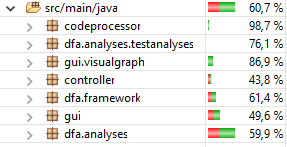
\includegraphics[width=0.8\textwidth]{Statistiken/coverage.png}
	\label{fig1}
\end{figure}


Hier wird lediglich die Abdeckung durch automatische Tests dargestellt. Zusätzlich dazu wurden noch manuelle Tests ausgeführt. Für diese stehen aber keine Überdeckungs-Statistiken zur Verfügung.
\end{document}